%======================================================================
%   D O C U M E N T   P R E A M B L E
\documentclass[letterpaper,12pt,titlepage,oneside,final]{book}

\newcommand{\package}[1]{\textbf{#1}}
\newcommand{\cmmd}[1]{\textbackslash\texttt{#1}}
\newcommand{\href}[1]{#1}
\usepackage{geometry}

% Set one-inch margins on all sides
\geometry{margin=1in}
% This package allows if-then-else control structures.
\usepackage{ifthen}
\newboolean{PrintVersion}
\setboolean{PrintVersion}{false}

\usepackage{mathptmx}

%\usepackage{subcaption}
% Bibliography
\usepackage[
	style=apa, % In-text citation style for APA, numeric otherwise
    giveninits=true,
]{biblatex}
\addbibresource{uw-ethesis.bib}

\usepackage{fancyhdr} % Required for customizing headers and footers
\usepackage{lastpage}
\usepackage{float}
\usepackage{amsmath,amssymb,amstext} % Lots of math symbols and environments
\usepackage[pdftex]{graphicx} % For including graphics N.B. pdftex graphics driver 

%---------------------------------------------
%	TABLES
%---------------------------------------------

\usepackage{booktabs} % Required for better horizontal rules in tables

\usepackage{array} % Required for manipulating table columns

\newcolumntype{R}[1]{>{\raggedleft\arraybackslash}p{#1}} % Define a new right-aligned paragraph column type
\newcolumntype{L}[1]{>{\raggedright\arraybackslash}p{#1}} % Define a new left-aligned (no justification) paragraph column type
\newcolumntype{C}[1]{>{\centering\arraybackslash}p{#1}} % Define a new centered paragraph column type

\usepackage[pdftex,pagebackref=false]{hyperref} % with basic options
%\usepackage[pdftex,pagebackref=true]{hyperref}
		% N.B. pagebackref=true provides links back from the References to the body text. This can cause trouble for printing.
\hypersetup{
    plainpages=false,       % needed if Roman numbers in frontpages
    unicode=false,          % non-Latin characters in Acrobat’s bookmarks
    pdftoolbar=true,        % show Acrobat’s toolbar?
    pdfmenubar=true,        % show Acrobat’s menu?
    pdffitwindow=false,     % window fit to page when opened
    pdfstartview={FitH},    % fits the width of the page to the window
    pdftitle={Explaining embedding results for scoring alignments},
    pdfauthor={Riley Gavigan},
    pdfsubject={Deep Learning},
    pdfkeywords={deep learning} {machine learning} {bioinformatics},       % list of keywords
    pdfnewwindow=true,      % links in new window
    colorlinks=true,        % false: boxed links; true: colored links
    linkcolor=blue,         % color of internal links
    citecolor=green,        % color of links to bibliography
    filecolor=magenta,      % color of file links
    urlcolor=cyan           % color of external links
}
\ifthenelse{\boolean{PrintVersion}}{   % for improved print quality, change some hyperref options
\hypersetup{	% override some previously defined hyperref options
%    colorlinks,%
    citecolor=black,%
    filecolor=black,%
    linkcolor=black,%
    urlcolor=black}
}{} % end of ifthenelse (no else)

\usepackage[automake,toc,abbreviations]{glossaries-extra}

% Setting up the page margins...
\setlength{\marginparwidth}{0pt} % width of margin notes
% N.B. If margin notes are used, you must adjust \textwidth, \marginparwidth
% and \marginparsep so that the space left between the margin notes and page
% edge is less than 15 mm (0.6 in.)
\setlength{\marginparsep}{0pt} % width of space between body text and margin notes
\setlength{\evensidemargin}{0in} % Adds 1/8 in. to binding side of all 
% even-numbered pages when the "twoside" printing option is selected
\setlength{\oddsidemargin}{0in} % Adds 1/8 in. to the left of all pages when "oneside" printing is selected, and to the left of all odd-numbered pages when "twoside" printing is selected
\setlength{\textwidth}{6.375in} % assuming US letter paper (8.5 in. x 11 in.) and side margins as above
\raggedbottom

% The following statement specifies the amount of space between paragraphs. Other reasonable specifications are \bigskipamount and \smallskipamount.
\setlength{\parskip}{\medskipamount}

% The following statement controls the line spacing.  
\renewcommand{\baselinestretch}{1}

\let\origdoublepage\cleardoublepage
\newcommand{\clearemptydoublepage}{%
  \clearpage{\pagestyle{empty}\origdoublepage}}
\let\cleardoublepage\clearemptydoublepage

\usepackage{titlesec}
\titlespacing*{\chapter}{0pt}{-35pt}{20pt}
\titleformat{\chapter}[display]
  {\normalfont\huge\bfseries}{}{0pt}{\Huge}

% Redefine the plain page style (used for chapter starting pages)
\fancypagestyle{plain}{
  \fancyhf{}
  \renewcommand{\headrulewidth}{0pt}
    \fancyhead[R]{\small\textit{Gavigan, Riley}}
    \fancyhead[L]{\small\textbf{Page \thepage{} of \pageref*{LastPage}}}
}

% Main glossary entries -- definitions of relevant terminology
\pagestyle{fancy}
\fancyhf{}
\renewcommand{\headrulewidth}{0pt}
\fancyhead[R]{\small\textit{Gavigan, Riley}}
\fancyhead[L]{\small\textbf{Page \thepage{} of \pageref*{LastPage}}}

\newglossaryentry{transformer}
{
name=transformer,
description={a type of neural network architecture used to solve the problem of transduction or transformation of input sequences into output sequences in deep learning applications using self-attention}
}

\newglossaryentry{amino acids}
{
name=amino acid,
description={molecules that combine to form proteins, containing both an amino and a carboxyl group}
}

\newglossaryentry{peptide}
{
name=peptide,
description={a compound consisting of two or more amino acids linked in a chain, the carboxyl group of each acid being joined to the amino group of the next},
plural={peptides}
}

\newglossaryentry{residue}
{
name=residue,
description={a single unit that makes up a polymer, such as an amino acid in a polypeptide chain},
plural={residues}
}

% List of Abbreviations
\newabbreviation{NLP}{NLP}{Natural Language Processing}
\newabbreviation{BLAST}{BLAST}{Basic Local Alignment Search Tool}
\newabbreviation{BERT}{BERT}{Bidirectional Encoder Representations from Transformers}
\newabbreviation{ALBERT}{ALBERT}{A Lite BERT}
\newabbreviation{RoBERTa}{RoBERTa}{Robustly Optimized BERT}
\newabbreviation{T5}{T5}{Text-To-Text Transfer Transformer}
\newabbreviation{ENNA}{ENNA}{Evolutionary Neural Network Algorithm}
\newabbreviation{MSA}{MSA}{Multiple Sequence Alignments}
\newabbreviation{LLM}{LLM}{Large Language Models}
\newabbreviation{LoRA}{LoRA}{Low-Rank Adaptation}
\newabbreviation{CDD}{CDD}{Conserved Domain Database}
\newabbreviation{BLOSUM}{BLOSUM}{BLOcks SUbstitution Matrix}
\makeglossaries
\begin{document}
% T I T L E   P A G E
\begin{titlepage}
        \begin{center}
        \vspace*{1.0cm}

        \Huge
        {\bf Explaining embedding results for scoring alignments }

        \large
        Final Progress Report \\

        \vspace*{1.0cm}

        \normalsize
        by \\

        \vspace*{1.0cm}

        \Large
        Riley Gavigan \\

        \vspace*{3.0cm}

        \normalsize
        CS 4490Z \\
        Thesis Supervisor: Lucian Ilie \\ 
        Course Instructor: Nazim Madhavi \\

        \vspace*{2.0cm}

        Department of Computer Science \\
        University of Western Ontario, London, N6A 5B7, Ontario, Canada \\
        \today \\

        \vspace*{1.0cm}
        \end{center}
\end{titlepage}

% Define a new chapter format that doesn't display the chapter number
\titleformat{\chapter}[display]
  {\normalfont\huge\bfseries}{}{0pt}{\Huge}

\setcounter{page}{2}

\cleardoublepage
\phantomsection

\printglossary

% L I S T   O F   A B B R E V I A T I O N S
\renewcommand*{\abbreviationsname}{Abbreviations}
\printglossary[type=abbreviations]
\cleardoublepage
\phantomsection

% A B S T R A C T
% ---------------
\chapter*{Structured Abstract}
\addcontentsline{toc}{chapter}{Structured Abstract}

\subsubsection*{Context and motivation}
The \textit{E}-score protein alignment scoring method \autocite{Ashrafzadeh:2023} outperforms state-of-the-art methods, supported by comparing ProtT5 \autocite{Elnaggar:2021} \textit{E}-score results with BLOSUM45 \autocite{Henikoff:1992}.

This research aimed to understand \textit{E}-score results, building upon the observation that mean cosine similarity results between two embeddings are not evenly distributed.

By understanding the underlying causes of the observed results, we can improve the \textit{E}-score method. Insights can be used to fine-tune the transformer models \autocite{Elnaggar:2021, Rives:2021} and performance of embeddings.

\subsubsection*{Research questions}
\begin{itemize}
    \item{What properties of embeddings produce better cosine similarity results?}
    \item{Why do cosine similarity results primarily fall within a positive range?}
    \item{How can models be fine-tuned to produce better embeddings?}
\end{itemize}

\subsubsection*{Principal ideas}
Positive cosine similarity results imply the produced embeddings are mostly similar. Comparing different embedding types provides insight into their distributions. Through these comparisons, conclusions about properties that improve \textit{E}-score results were drawn.

\subsubsection*{Research methodology}
This research is a data science investigation to obtain insight about the embeddings and cosine similarity results in the \textit{E}-score method.

\subsubsection*{Anticipated results}
This study primarily aimed to obtain insight and knowledge for the \textit{E}-score method, specifically:
\begin{itemize}
    \item{Knowledge about the distributions of different embedding types}
    \item{Knowledge about the cosine similarity between embeddings}
    \item{Insight to fine-tune and improve models}
\end{itemize}

\subsubsection*{Novelty}
By building upon a novel method for scoring protein alignments using cosine similarity \autocite{Ashrafzadeh:2023}, novel conclusions about embeddings and cosine similarity were made, leading to further research that can improve embeddings and models.

\subsubsection*{Impact}
Improvements in transformer models for the \textit{E}-score alignment scoring method can be made through the insight this research found. Improvements may also be applicable to \gls{NLP} Models such as T5 \autocite{Raffel:2020}.

\subsubsection*{Progress and completed work}
Insight into properties behind embedding type distributions was obtained. From these properties, cosine similarity results were explained. These properties were explained through conducted research and simulation in combination with insight from biochemical background research.

\subsubsection*{Limitations}
No limitations are known to exist in this research.

\cleardoublepage
\phantomsection

% T A B L E   O F   C O N T E N T S
% ---------------------------------
\renewcommand\contentsname{Table of Contents}
\tableofcontents
\cleardoublepage
\phantomsection

% L I S T   O F   S Y M B O L S
% ---------------------------
\cleardoublepage
\phantomsection

% Change page numbering back to Arabic numerals
\pagenumbering{arabic}
 

\setcounter{page}{8}
\chapter{Introduction}
Proteins are one of the four molecules of life. Finding similarities among protein sequences is essential in identifying protein structure and function. This is done by computing alignments between sequences.

The \textit{E}-score method is a method computes alignments between sequences using contextual embeddings produced by \gls{transformer} models (\cite{Ashrafzadeh:2023}). This method uses several different transformer models based off of \gls{NLP} models (\cite{Devlin:2018, Zhenzhong:2020, Liu:2019, Yang:2022, Raffel:2020}).

These transformer models produce embeddings when provided protein sequences. Understanding the values and distributions of these embeddings between each model is one focus of this research (\hyperlink{O1}{O1}).

\textit{E}-score uses cosine similarity to compute similarity between pairs of embeddings for scoring alignments. This research analyzes the distributions of observed cosine similarity results for natural and random protein sequences (\hyperlink{O2}{O2}, \hyperlink{O3}{O3}).

Combining embedding distribution and cosine similarity results with biochemical understandings of proteins is used to draw conclusions about model performance and \textit{E}-score results. Specifically, explanations about why some models outperform other models are derived (\hyperlink{O1}{O1}, \hyperlink{O2}{O2}).

Using inference about the proposed factors contributing to \textit{E}-score performance, I describe the procedure and techniques for fine-tuning ProtT5 to produce better embeddings for the \textit{E}-score method (\hyperlink{O4}{O4}).

\noindent Significant results from this research include:
\begin{itemize}
    \item{Significant positive correlation between higher embedding value variance and improved \textit{E}-score performance for a given model.}
    \item{Significant positive correlation between average cosine similarity results approaching 0 and improved \textit{E}-score performance for a given model.}
\end{itemize}

Novel implications about model flexibility and fine-tuning models to better adapt to the frequency of \glspl{residue} (or words in \gls{NLP}) provide significant insight into improving performance of different models for not only \textit{E}-score, but for any method using \glspl{transformer}.

\section{Report structure}
Chapter 2 provides a reader with background on important concepts and details discussed later in the thesis. Chapter 3 outlines the objectives of the research. Chapter 4 outlines the materials and methods used in the research conducted on the \textit{E}-score method. Chapter 5 provides the results from analysis performed in the data science investigation. Chapter 6 discusses the results, their implications, limitations, and generalizations. Chapter 7 concludes the study by addressing the research questions outlined in the thesis proposal, and discusses impact and novelty of the results. Chapter 8 discusses potential future work and novel lessons learned from this research.
\chapter{Background and Related Work}

\section{Natural Language Processing}
Natural Language Processing is the branch of artificial intelligence that deals with computers understanding text and spoken words (\cite{Khurana:2023}). One significant advancement was the introduction of \glspl{transformer} (\cite{Vaswani:2017}). Before Transformers, methods such as word2vec (\cite{Mikolov:2013}) and GloVe (\cite{Pennington:2014}) generated contextually-independent embedding vectors for words. Transformer models introduced contextual embeddings generated through self-attention (\cite{Vaswani:2017}).

\noindent Information about each model serving as foundation for \textit{E}-score models:
\begin{itemize}
    \item{\gls{T5}: Text-to-text approach. Input and output are both text strings. Relies of transfer learning for downstream fine-tuning (\cite{Raffel:2020}). GLUE benchmark average: 88.7}
    \item{\gls{BERT}: Bidirectional training using masked language modeling for a deeper sense of context from sequential reading (\cite{Devlin:2018}).}
    \item{\gls{ALBERT}: A lightweight version of BERT that uses parameter-reduction techniques to reduce training time and memory limitations (\cite{Zhenzhong:2020}). GLUE benchmark average: 87.3}
    \item{\gls{RoBERTa}: A stronger version of BERT that was trained longer; removed next-sentence pretraining; and trained with larger mini-batches and learning rates (\cite{Liu:2019}). GLUE benchmark average: 86.4}
    \item{XLNet: Designed to overcome the pretrain-finetune discrepency BERT suffered from, outperforming BERT significantly on 20 tasks (\cite{Yang:2022}). GLUE benchmark average: 87.5}
\end{itemize}

\section{\textit{E}-score}
Finding similarities among protein sequences is essential in identifying protein structure and function. This is done by computing alignments between sequences. The \gls{BLAST} program\footnote{Exceeds 108,000 citations, according to Google Scholar.} is one of the most widely used tools in science (\cite{Atschul:1990}). An essential part of BLAST is the scoring function; the most widely used functions are provided by the \gls{BLOSUM} (\cite{Henikoff:1992}).

The \textit{E}-score protein alignment scoring method (\cite{Ashrafzadeh:2023}) is another one of these scoring functions that outperforms state-of-the-art methods. \textit{E}-score's improved performance was supported by comparing ProtT5 (\cite{Elnaggar:2021}) results with BLOSUM45 (\cite{Henikoff:1992,Ashrafzadeh:2023}). \textit{E}-score uses \gls{transformer} models to produce contextual embeddings for the \glspl{residue} in \gls{peptide} sequences. Model information is available in Table \ref{tab:prottrans}.

Contextual embeddings describe the position of a \gls{residue} in a high-dimensional vector space. Contextual embeddings have many important applications in biology, including structure prediction (\cite{Senior:2020, Yang:2019, Jumper:2021}) and function prediction (\cite{Kulmanov:2019, Gligorijevic:2021, Lai:2021}). The \textit{E}-score alignment method is another application for these embeddings, outperforming the state-of-the-art methods (\cite{Ashrafzadeh:2023}) by completely changing the way alignments are computed.

The embedding vector produced for each protein \gls{residue} varies based on the model. Embedding dimensions and pre-training dataset are outlined in the \href{https://github.com/rgavigan/e-score/blob/main/README.md}{research code repository}. The dimensionality of the embedding vectors represents the number of features encoded in the embedding, and is a fixed value for each model.

Calculating the cosine similarity between two vectors \(A = (A_i)_{i=1..n}\) and \(B = (B_i)_{i=1..n}\): \(\frac{A \cdot B}{\Vert A \Vert \Vert B \Vert}\). \textit{E}-score is calculated by taking the cosine similarity between the embedding vectors from two \glspl{residue}.

In calculating sequence alignment using the \textit{E}-score method, the cosine similarity results were mostly mostly less than \(\frac{\pi}{2}\). ProtT5 had the best performance (\cite{Ashrafzadeh:2023}).

\section{Analysis and Research Gap}
There is no research analyzing results and properties contributing to improved embedding performance for comparable models to the \textit{E}-score method using protein transformers. Fine-tuning \gls{LLM} is a powerful technique to leverage pre-trained models and adapt them to perform better at a specific task or tasks. Fine-tuning can be improved upon using insights such as those taken from this research. The purpose of fine-tuning is to avoid the need to pre-train a model from scratch for a task; instead relying on powerful pre-trained models and modifying them to better suit the task.

Supervised learning involves providing the model with a labeled dataset, and the model will learn to map the input to the output by minimizing its loss function (\cite{Mohri:2018}). Reinforcement learning involves providing a reward signal to the model when it generates a desired output, and the model learns to generate the desired output for a task by maximizing the reward signal (\cite{Sutton:1998}). Both of these tasks can be leveraged along with novel conclusions from this research to better fine-tune models for \textit{E}-score and for other tasks that follow similar procedures to draw unique conclusions. Fine-tuning techniques such as \gls{LoRA}, a technique that freezes the pre-trained weights and injects a trainable rank decomposition matrix into each layer of the architecture, can minimize compute intensity of fine-tuning procedures that this research can lead to.
\chapter{Research Objectives}
\begin{itemize}
    \item{\hypertarget{O1}{O1}: Understand the reasoning behind the observed distributions of different embedding types. Explaining both individual and relative results for \textit{E}-score models.}
    \item{\hypertarget{O2}{O2}: Understand what properties of embeddings help produce better cosine similarity and alignment results.}
    \item{\hypertarget{O3}{O3}: Understand why cosine similarity results primarily fall within a positive range.}
    \item{\hypertarget{O4}{O4}: Determine how models can be fine-tuned to improve \textit{E}-score method results.}
\end{itemize}
\chapter{Methodology}

\section{Protein composition}
Proteins are not completely random in nature. By determining the frequencies of amino acids in our dataset of protein sequences, we showcase that there is not an equal distribution of amino acids present in nature. We also use these frequencies to perform a simulation on completely random proteins for a given length \(n\) of a polypeptide. By simulating every combination and calculating the cosine similarity for a given length of proteins using only the frequency of amino acids as a constraint, we are able to outline one factor contributing to observed cosine similarity results (\hyperlink{O1}{O1}).

\section{Embeddings and cosine similarity}
By applying the above analysis and further supporting it with more properties of proteins such as their secondary structures, we analyze and explain why cosine similarity results are mostly positive (\hyperlink{O2}{O2}, \hyperlink{O3}{O3}). Similar to how in \gls{NLP} we would observe documents having similar sentences (ex: e-mails always contain a selection of entry and closing statements such as "Good morning" and "Warm regards"), the rules that proteins follow would result in similarities between sequences.

To support findings from embedding vector and cosine similarity analysis, background knowledge about the properties of different models is used to explain the performance differences (\hyperlink{O1}{O1}). Table \ref{tab:prottrans} highlights some key properties about the models available in the \textit{E}-score method.

Results from the papers proposing each model are used to support findings in Chapter 5 (\hyperlink{O4}{O4}). Details regarding ProtTrans models, ESM-1b, and ESM2 are found in their respective papers (\cite{Elnaggar:2021, Elnaggar:2022, Rives:2021, Rao:2020, Lin:2022}).

Empirical procedures involve obtaining and collecting data for natural and random protein sequences, using them as input for each model, and collecting information about embedding vector distributions and cosine similarity between embedding vectors for every generated embedding. Findings are validated through t-tests to determine statistical significance of results for embeddings and cosine similarity.

Source code for these empirical procedures used to generate results is \href{https://github.com/rgavigan/e-score/blob/main/src/e-score.ipynb}{located on GitHub}. Empirical procedures use the following: embedding generation for selected sequences; normalization of embedding values for comparison; averaging embedding values for different models for both random and non-random sequences; and averaging cosine similarity between embeddings for both random and non-random sequences.

\chapter{Results}

\section{Data}
Data was obtained through the \gls{CDD} for different \glspl{MSA} from the list of 49 selected in the \textit{E}-score paper (\cite{Marchler-Bauer:2015, Ashrafzadeh:2023}). Selected \glspl{MSA} are found in Table \ref{tab:msa} and in the \href{https://github.com/rgavigan/e-score/tree/bf08fa86209a6ce9956d48212690b1814450e72b/data/finetuning/msa-proteins}{code repository}.

\begin{table*} % Two column table
	\caption{10 MSAs with the most proteins from CDD used in the \textit{E}-score comparison procedure (\cite{Ashrafzadeh:2023, Marchler-Bauer:2015}).}
	\centering
    \vspace{2mm}
    \scalebox{0.9}{
	\begin{tabular}{ lrrr }
		\toprule
        \multicolumn{4}{c}{MSAs} \\
        \midrule
		Conserved Domain & Source & Proteins & Length \\
		\midrule
        \(CS\_CSD\) & cd00024 & 522 & 98 \\
        \(7tm\_classA\_rhodopsin\-like\) & cd00637 & 405 & 808 \\
        \(FYVE\_like\_SF\) & cd00065 & 392 & 266 \\
        \(Mb\-like\) & cd01040 & 384 & 239 \\
        \(SH2\) & cd00173 & 352 & 214 \\
        \(C1\) & cd00029 & 281 & 99 \\
        \(KAZAL\_FS\) & cd00104 & 273 & 74 \\
        \(Globin\_sensor\) & cd01068 & 193 & 223 \\
        \(Bbox2\) & cd19756 & 127 & 65 \\
        \(NBD\_sugar\-kinase\_HSP70\_actin\) & cd00012 & 125 & 1154 \\
		\bottomrule
	\end{tabular}
    }
	\label{tab:msa}
\end{table*}

\noindent Procedure for obtaining CDD MSA data:
\begin{enumerate}
    \item{Select a source from Table \ref{tab:msa}.}
    \item{Search for the source on the \href{https://www.ncbi.nlm.nih.gov/cdd}{CDD website}.}
    \item{Click 'Representatives' under 'Links', send to FASTA format.}
    \item{For reference alignments: click 'Download Alignment' instead of going to 'Representatives'}
\end{enumerate}

\noindent Alignment pairs \(i, j\) were enumerated by iterating through each FASTA file: \(\forall i~\forall j, ~i \ne j\). These pairs were used to determine embedding value distributions (\hyperlink{O1}{O1}) and cosine similarity distributions (\hyperlink{O3}{O3})  for natural proteins. Reference alignments serve as necessary data for future fine-tuning efforts based on drawn conclusions.

Random sequence data was generated by randomly selecting \glspl{residue} of equal probability with replacement for sequences of random lengths between 100 and 400. This data was used to compare random embeddings and cosine similarity to naturally-observed results (\hyperlink{O1}{O1}).

\section{Protein composition}

Sequence similarity is essential in sequence analysis within bioinformatics (\cite{Ofer:2021}). Peptide sequence alignment is the most complex case, with a language of 20 common \glspl{amino acids} forming a theoretically countably infinite amount of unique \gls{peptide} sequences shown in Equation \ref{eq:peptideinfinity} by taking the n-ary Cartesian product.

\begin{equation}
    {Theoretical\, Limit} = \prod_{k=1}^{\infty} |A| = \prod_{k=1}^{\infty} 20 = 20 \times 20 \times \ldots
    \label{eq:peptideinfinity}
\end{equation}

Observed sequences in living organisms are constrained by biological, genetic, and functional factors. For example, the average eukaryotic protein size is $353 \pm 62.5$ \glspl{residue} (\cite{Nevers:2023}). 

Databases such as UniProt (\cite{UniProt:2023}) and PeptideAtlas (\cite{PeptideAtlas:2006}) are repositories filled with \gls{peptide} sequences. UniProt contains over 250 million unique peptide sequences and counting (\cite{UniProt:2023}).

Peptide sequences are not completely random because of the constraints imposed on them. Similar to letters or words in a given language within natural language, the frequency of each \gls{amino acids} observed in nature is not equally distributed (\cite{Beals:1999}).

Proteins form secondary structures as part of larger tertiary and quaternary structures. The most common of these secondary structures are \(\alpha\) helices and \(\beta\) pleated sheets (\cite{Ma:2018}). Because of this, algorithms such as an \gls{ENNA} are able to distinguish natural proteins from randomly generated proteins with an accuracy of over 94\% (\cite{Lucrezia:2012}).

The distribution of the observed amino acids in all of the protein sequences from the 10 MSAs in Table \ref{tab:msa} is shown in Table \ref{tab:aadist}. Counts were acquired by reading FASTA file sequences for each MSA and generating a \LaTeX~table containing names, frequencies, and percentages for the 20 most common \glspl{amino acids}.

\begin{table}[H] % Two column table
	\caption{Distribution of amino acids found in the 10 selected MSAs. A few occurrences of 'B' (nondeterministically either N or D) and some occurrences of 'X' (undetermined or atypical amino acid) were left out for simplicity.}
	\centering
    \vspace{2mm}
    \begin{tabular}{lrrrrl}
    \toprule
     Amino Acid & Symbol & Frequency & Percent & Diff From Equal & P-value \\
    \midrule
    Leucine & L & 152859 & 9.099 & 4.099 & 0.0e+00 \\
    Serine & S & 141844 & 8.443 & 3.443 & 0.0e+00 \\
    Alanine & A & 127926 & 7.614 & 2.614 & 0.0e+00 \\
    Glutamic Acid & E & 108476 & 6.457 & 1.457 & 0.0e+00 \\
    Valine & V & 105408 & 6.274 & 1.274 & 0.0e+00 \\
    Arginine & R & 99687 & 5.934 & 0.934 & 3.2e-293 \\
    Glycine & G & 96906 & 5.768 & 0.768 & 3.6e-202 \\
    Threonine & T & 96702 & 5.756 & 0.756 & 4.1e-196 \\
    Lysine & K & 94251 & 5.610 & 0.610 & 3.6e-130 \\
    Aspartic Acid & D & 88980 & 5.296 & 0.296 & 5.2e-33 \\
    Isoleucine & I & 87579 & 5.213 & 0.213 & 5.9e-18 \\
    Proline & P & 86463 & 5.146 & 0.146 & 2.5e-09 \\
    Glutamine & Q & 74206 & 4.417 & 0.583 & 6.3e-134 \\
    Asparagine & N & 73490 & 4.374 & 0.626 & 1.3e-154 \\
    Phenylalanine & F & 64495 & 3.839 & 1.161 & 0.0e+00 \\
    Tyrosine & Y & 46324 & 2.757 & 2.243 & 0.0e+00 \\
    Histidine & H & 43163 & 2.569 & 2.431 & 0.0e+00 \\
    Cysteine & C & 36749 & 2.187 & 2.813 & 0.0e+00 \\
    Methionine & M & 35289 & 2.100 & 2.900 & 0.0e+00 \\
    Tryptophan & W & 19243 & 1.145 & 3.855 & 0.0e+00 \\
    \bottomrule
    \end{tabular}
	\label{tab:aadist}
\end{table}

\section{\textit{E}-score model differences}
The \gls{transformer} models used in the \textit{E}-score method (see Table \ref{tab:transformers}) vary in performance (\hyperlink{O1}{O1}). ProtT5 outperformed the 5 other models available when computing end-gap-free alignments for six different conserved domain \glspl{MSA}. ProtT5 and ESM2, the second best model, were compared and it was evident that ProtT5 outperformed ESM2 with statistically significant results (\cite{Ashrafzadeh:2023}).

\textit{E}-score's protein transformers models have significantly different pre-training configurations (\cite{Elnaggar:2021, Rives:2021}), some of which are highlighted in Table \ref{tab:prottrans} (\hyperlink{O1}{O1}).

\begin{table*} % Two column table
	\caption{Pre-training configuration for protein language models (\cite{Elnaggar:2021,Rives:2021}). UR = UniRef.}
	\centering
	\begin{tabular}{ lllllll }
		\toprule
		Hyperparam & ProtT5 & ProtBert & ProtXLNet & ProtAlbert & ESM1b & ESM2 \\
		\midrule
		Dataset & UR50 & UR100 & UR100 & UR100 & UR50 & UR50 \\
		\# of Layers & 24 & 30 & 30 & 12 & 33 & 33 \\
		Embedding Dim & 1024 & 1024 & 1024 & 4096 & 1280 & 1280 \\
        \# of Params & 3B & 420M & 409M & 224M & 650M & 650M \\
        Learning Rate & 0.01 & 0.002 & 0.00001 & 0.002 & 0.0004 & 0.0004 \\
		\bottomrule
	\end{tabular}
	\label{tab:prottrans}
\end{table*}

Protein transformer model pre-training configurations significantly impact model performance. For example, ProtT5 has 3 billion parameters compared to ProtAlbert having 224 million. Model performance and number of parameters are highly correlated, which is supported by the Chinchilla paper's findings for training compute-optimal \glspl{LLM} (\cite{Hoffman:2022}). Through the results from the comparison between models in the \textit{E}-score paper (\cite{Ashrafzadeh:2023}), it was evident that the encoder-decoder model ProtT5 outperformed both the encoder-only models (ESM1b, ESM2, ProtBert, ProtAlbert) and the decoder-only model (XLNet).

\section{Embeddings}
Understanding embedding distributions is crucial in understanding cosine similarity results and how they can be improved (\hyperlink{O2}{O2}). Embedding distributions were compared for all ProtTrans models in the \textit{E}-score method for both randomly selected natural protein sequences and randomly generated sequences. Embedding value distributions are visualized in Figure \ref{fig:embedding_avg}.     The procedure for obtaining average embedding values is described below:
\begin{itemize}
    \item{Obtain n sequences to provide as input to a model}
    \item{Produce and store the embedding values for all n sequences}
    \item{Normalize the embedding values, then obtain the average and standard deviation of all n embeddings}
\end{itemize}

\begin{figure}[H]
    \begin{center}
	   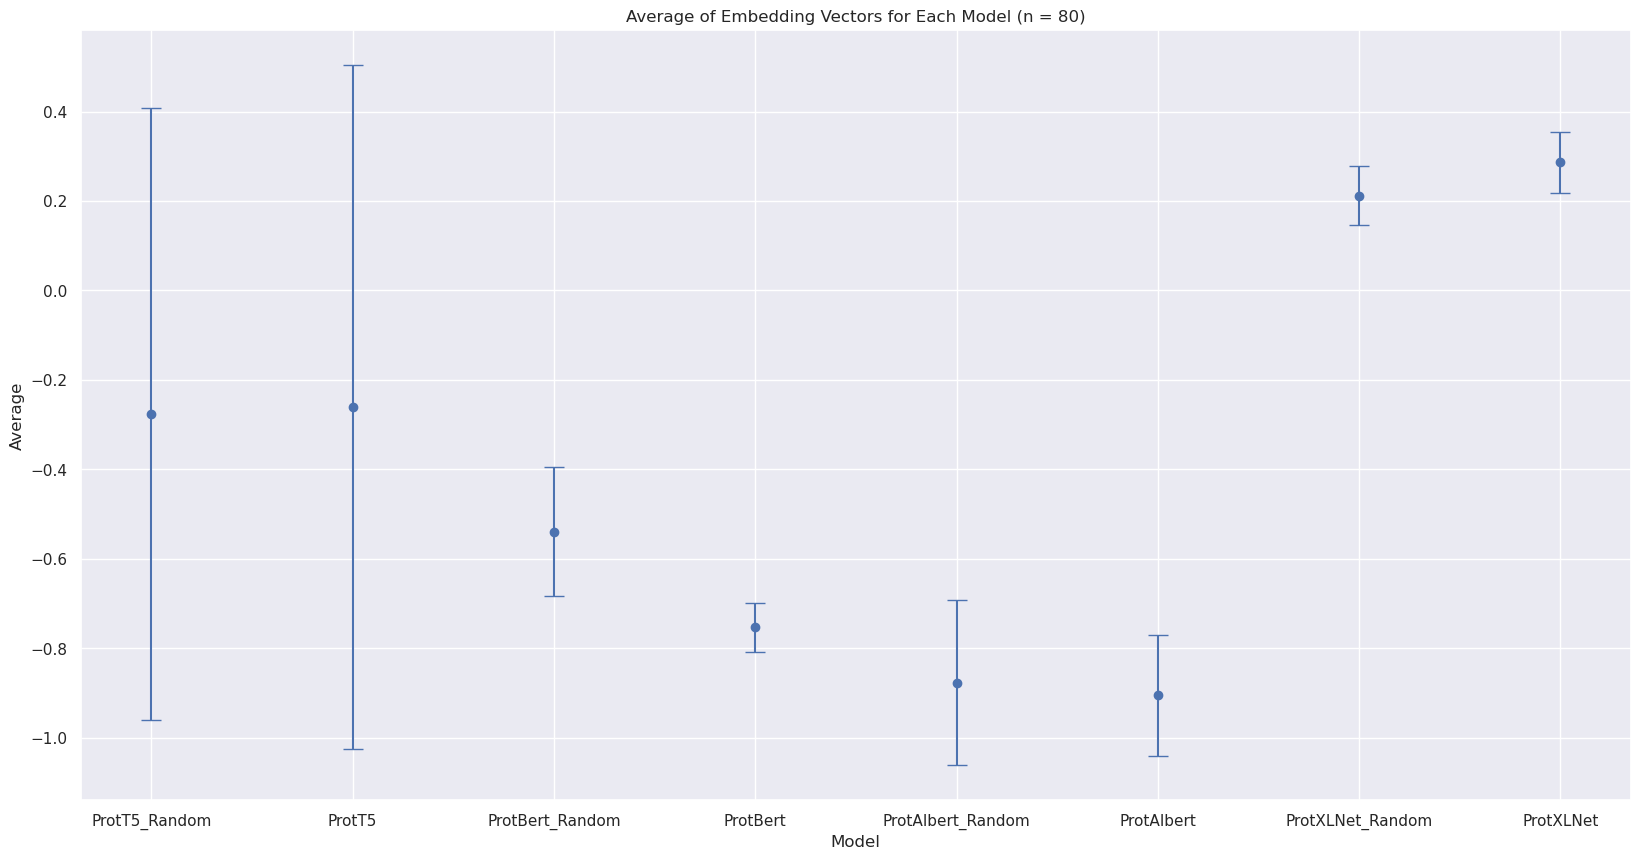
\includegraphics[width=0.9\linewidth]{figures/embedding_avg.png}
    \end{center}
    \caption{Average embedding values for 80 random and non-random (randomly chosen from CDD) embeddings for all ProtTrans models. Values scaled to -1...1.}
    \label{fig:embedding_avg}
\end{figure}

\section{Cosine Similarity}
Cosine similarity distributions were compared for all ProtTrans models in the \textit{E}-score method for randomly selected natural protein sequences and randomly generated sequences. Cosine similarity distributions are visualized in Figure \ref{fig:random_vs_nonrandom_cossim}. The procedure for determining cosine similarity distributions is described below:
\begin{itemize}
    \item{Get embeddings for n sequences from a selected model.}
    \item{Calculate the cosine similarity between every pair \(i, j\) of embeddings, for a total of \(n^2\) cosine similarity calculations.}
\end{itemize}


\begin{figure}[H]
    \begin{center}
	   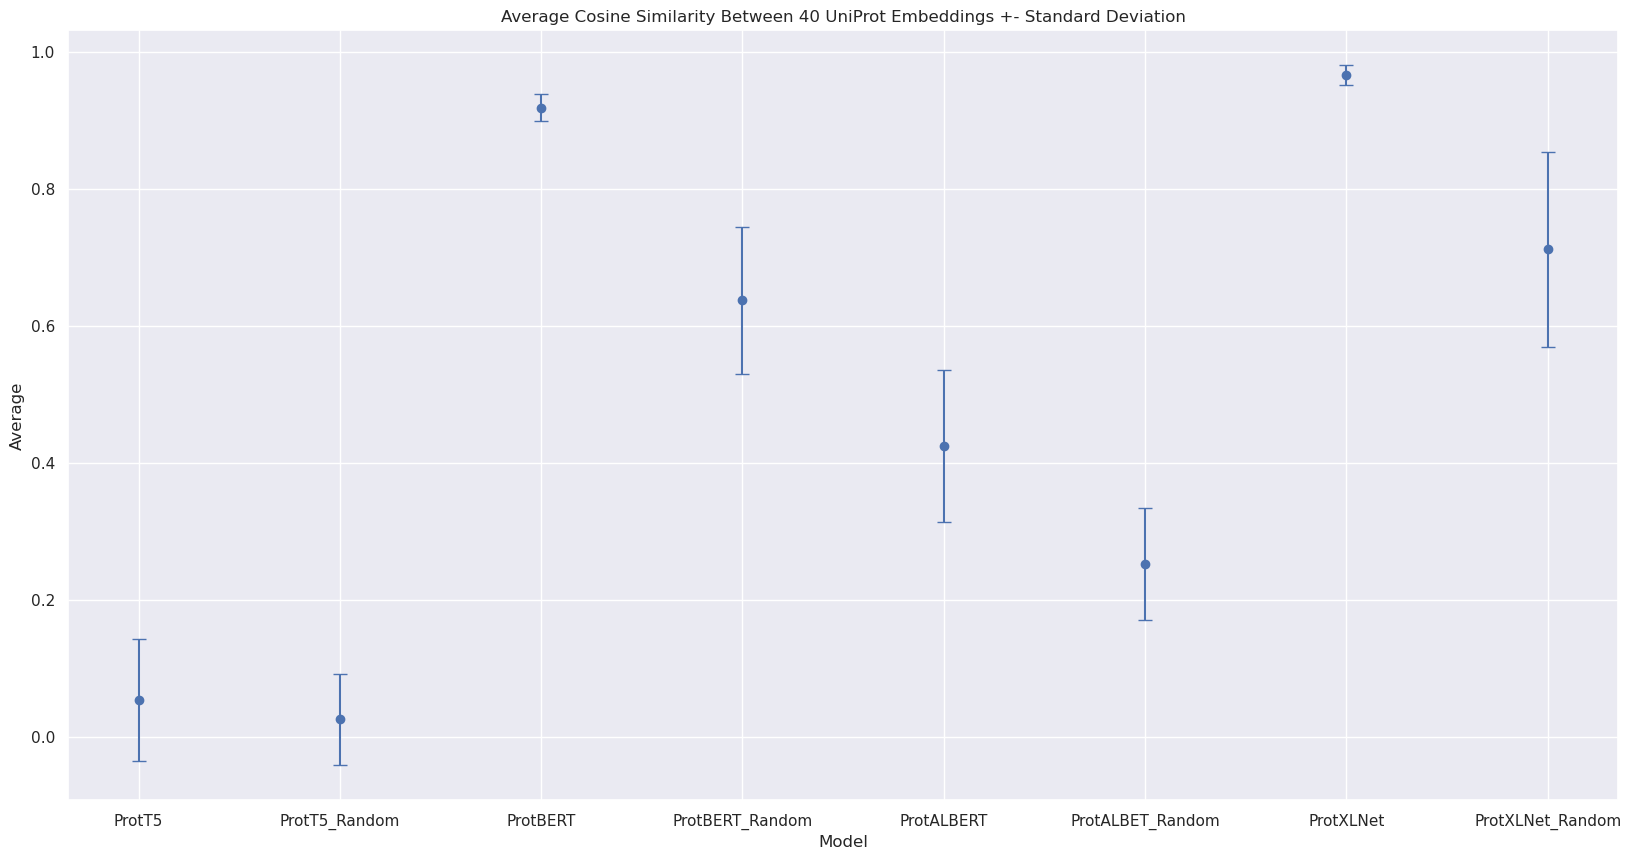
\includegraphics[width=1.0\linewidth]{figures/random_vs_nonrandom_cossim.png}
    \end{center}
    \caption{Average cosine similarity between sample and random embeddings for all ProtTrans models. P-Values are all \(0.000\) between any column and overall average of 0.59 (and between any chosen comparison).}
    \label{fig:random_vs_nonrandom_cossim}
\end{figure}

\chapter{Discussion}

\section{Implications}
The results derive implications that can be used to enhance the \textit{E}-score method with \gls{LoRA} fine-tuning. This is primarily applicable to ProtT5, as it is the best-performing method with pre-made fine-tuning notebooks that can expanded upon, but is also applicable to other models. We can fine-tune the other models to catch up to ProtT5's performance by generating embeddings with more variance in their average values. Additionally, we can create a custom penalty function to punish these models for producing mostly similar cosine similarity results, bringing the average cosine similarity result closer to 0 and closer to ProtT5's average.

The connection between observations in nature and embedding results from models is highly evident from this research. Most models fail to capture variance because of these laws governing nature, which ProtT5 managed to overcome (likely only because of its size) as results in Section 5.4 outlined. AlphaFold (\cite{Jumper:2021}) is a protein structure prediction method developed by Google DeepMind that uses protein transformers as the E-score method does. Because we are able to predict protein structure with transformers, it is evident that primary structures, secondary structures, structural motifs, and other properties of proteins are heavily correlated. Results from Section 5.1 and 5.2 further support this claim and outline the importance of adapting models to account for these rules. More efficient training strategies can be researched to improve the performance of models despite identical size and training time (more compute-optimal).

\section{Limitations and Generalizations}
Limited compute power (GPU: RTX 4070 Super) impacted the scale of embedding distribution and cosine similarity distribution procedures. With more compute power, these procedures could be conducted for all 49 \glspl{MSA} used in the \textit{E}-score method and an equivalent number of random sequences. This would greatly improve the validity of the results.

% Generalizability
Results are generalizable to other systems utilizing ProtTrans, ESM-1b, and ESM2 models (\cite{Elnaggar:2021, Rives:2021}). Novel conclusions can be used to support fine-tuning models for their respective use-cases. \gls{NLP} use cases may repeat experimental procedures in future research to determine word frequency (ex: the word "what" is much more common in English than "myriad"), embedding distribution (\hyperlink{O1}{O1}), and their correlation with the results of a respective method (such as \textit{E}-score's \hyperlink{O3}{O3}) to find parallel conclusions.
\chapter{Conclusions}
This study aimed to address the limited insight into factors that contribute to better model performance in the \textit{E}-score alignment method (\cite{Ashrafzadeh:2023}). Objectives included understanding embedding distributions for models and for both random and non-random sequences (\hyperlink{O1}{O1}, \hyperlink{O2}{O2}); understanding cosine similarity between these embeddings(\hyperlink{O3}{O3}); and determining how we can improve models in task performance (\hyperlink{O4}{O4}). 

\noindent Key results and conclusions:
\begin{enumerate}
    \item{Proteins are not random in nature. Amino acid frequencies are not equal and vary to form particular secondary, tertiary, and quaternary structures. The reference MSAs contain significantly different frequencies for all 20 common amino acids (Section 5.2).}
    \item{\textit{E}-score model performance is correlated heavily with the size of a model. This is supported by ProtT5 (3 billion parameters) outperforming every other model, with ESM2 performing second best (650 million parameters) (Section 5.3).}
    \item{Embedding value distributions with a higher variance perform better in the \textit{E}-score method. This is supported by ProtT5 significantly outperforming all other models with a much higher variance. For worst performing models, variance is constrained by the non-random nature of proteins with random sequences having a significantly higher variance (Section 5.4).}
    \item{Cosine similarity distributions are heavily correlated with model performance. ProtT5, the best method, has an average cosine similarity close to 0. All other models over-represent positive cosine similarity results, implying that they fail to capture variation as well as ProtT5 (Section 5.5).}
\end{enumerate}
\chapter{Future Work and Lessons Learned}
Using the ProtTrans \href{https://github.com/rgavigan/e-score/blob/fae7672033f51adc77030f33a62d16ab415d17f5/src/fine-tune-t5-per-protein.ipynb}{per-protein fine-tuning notebook} as a basis to fine-tune ProtT5 for the \textit{E}-score method may lead to significant performance benefits, especially if modified for other models. This requires significant modifications to the fine-tuning process:
\begin{itemize}
    \item{Fine-tune the model with the ProtT5 per-protein notebook as a basis, creating a LoRA adapter for the \textit{E}-score method.}
    \item{Modify the fine-tuning notebook to work on pairs of inputs as opposed to a singular input, with penalties being assigned based on how far the \textit{E}-score alignment score for the pair of embeddings is from the true reference alignment.}
\end{itemize}

\noindent Significant lessons learned from this research:
\begin{enumerate}
    \item{Higher variance in produced embeddings is highly correlated to improved performance, meaning highly flexible models may be the key to improved \textit{E}-score performance.}
    \item{Average cosine similarity results closer to 0 are highly correlated with better \textit{E}-score performance. Models that make use of the full -1...1 cosine similarity range with better-produced embeddings perform better than those with mostly positive results. Fine-tuning models to reach a mean of 0 is likely to lead to better performance.}
    \item{The rules governing protein sequences observed in the world lead to higher cosine similarity results in all cases. Fine-tuning models to better capture variation while accounting for these properties (i.e. amino acid frequency) may lead to stronger results.}
\end{enumerate}

\section{Acknowledgements}
Dr. Lucian Ilie provided feedback on the thesis proposal and guidance throughout the process to conduct research following the original \textit{E}-score paper (\cite{Ashrafzadeh:2023}).

% Bibliography
\cleardoublepage
\phantomsection
\renewcommand*{\bibname}{References}
\addcontentsline{toc}{chapter}{\textbf{References}}
\printbibliography[heading=subbibliography]
%\nocite{*} % uncommenting will add references that werent cited in the document to it

\cleardoublepage
\phantomsection
%----------------------------------------------------------------------
\end{document} % end of logical document
